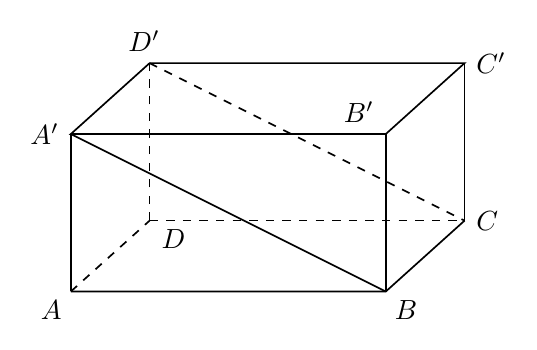
\begin{tikzpicture}[x=1cm,y=1cm,line width=0.6pt]
\tikzset{ptlabel/.style={font=\normalsize,fill=none,inner sep=1pt}}
\coordinate (A) at (0,0);
\coordinate (B) at (4,0);
\coordinate (C) at (5,0.9);
\coordinate (D) at (1,0.9);
\coordinate (Ap) at (0,2);
\coordinate (Bp) at (4,2);
\coordinate (Cp) at (5,2.9);
\coordinate (Dp) at (1,2.9);
% bottom and top faces
\draw[draw=black] (A)--(B)--(C);
\draw[draw=black] (Ap) -- (Bp) -- (Cp) -- (Dp) -- cycle;
% vertical edges
\draw[draw=black] (A) -- (Ap);
\draw[draw=black] (B) -- (Bp);
\draw[draw=black] (C) -- (Cp);
% hidden edges dashed
\draw[draw=black,dashed] (A) -- (D);
\draw[draw=black,dashed] (D) -- (Dp);
\draw[draw=black,dashed] (D) -- (C);
% face diagonal A'B solid, interior diagonal A'C dashed
\draw[draw=black] (Ap) -- (B);

\draw[draw=black,dashed] (Dp) -- (C);
% labels with clearance
\node[ptlabel,anchor=north east,xshift=-2pt,yshift=-2pt] at (A) {$A$};
\node[ptlabel,anchor=north west,xshift=2pt,yshift=-2pt] at (B) {$B$};
\node[ptlabel,anchor=west,xshift=3pt] at (C) {$C$};
\node[ptlabel,anchor=north west,xshift=3pt,yshift=-2pt] at (D) {$D$};
\node[ptlabel,anchor=east,xshift=-3pt] at (Ap) {$A'$};
\node[ptlabel,anchor=south east,xshift=-3pt,yshift=3pt] at (Bp) {$B'$};
\node[ptlabel,anchor=west,xshift=3pt] at (Cp) {$C'$};
\node[ptlabel,anchor=south,xshift=-2pt,yshift=3pt] at (Dp) {$D'$};
\end{tikzpicture}
